\title{第八周作业}
\author{洪艺中}
\maketitle
\section{第一部分}

\subsection*{ 106页 题目2 }
\begin{problem*}
设平行四边形的三个顶点的径向量分别为 $\mlr_1$, $\mlr_2$, $\mlr_3$, 求第四个顶点的径向量和对角交点的径向量用 $\mlr_1$, $\mlr_2$, $\mlr_3$ 表示的关系式.
\end{problem*}
\begin{solution}
平行四边形一共有四个顶点, 给出三个顶点之后还剩下一个需要确定的顶点. 因为题目中没有给定三个顶点的相对关系, 我们假设 $\mlr_\alpha$ ($\alpha \in \{1, 2, 3\}$) 在第四个顶点的对位, $\mlr_\beta$, $\mlr_\gamma$ ($\beta, \gamma \in \{1, 2, 3\}$ 且 $\{\alpha, \beta, \gamma\} = \{1, 2, 3\}$) 则在邻位. 那么
第四个顶点的径向量可以表示为
\[
    \mlr_\alpha + (\mlr_\beta - \mlr_\alpha) + (\mlr_\gamma - \mlr_\alpha) = \mlr_\beta + \mlr_\gamma - \mlr_\alpha,
\]
对角线的交点则是平行四边形的中心. 根据之前作业题(习题 4.1 题目 5)的结论, 其径向量为
\[
    \frac{1}{4}[\mlr_\alpha + \mlr_\beta + \mlr_\gamma + (\mlr_\beta + \mlr_\gamma - \mlr_\alpha)] = \frac{1}{2}(\mlr_\beta + \mlr_\gamma).
\]
\end{solution}

\subsection*{ 题目 5 }
\begin{problem*}
    判断向量组是否共面. 题目略.
\end{problem*}
\begin{solution}
    判断是否共面, 只需计算三个向量构成的平行六面体的体积:
    \begin{enumerate}
        \item[(1)]
        \[
        \left|
            \begin{matrix}
                \mla^\top & \mlb^\top & \mlc^\top
            \end{matrix}
        \right| = 
        \left|
            \begin{matrix}
                 0 & 1 & 2 \\
                -1 & 1 & 1 \\
                 2 & 3 & -1
            \end{matrix}
        \right| = -9.
        \]
        因此三个向量不共面.
        \item[(2)] \[
        \left|
            \begin{matrix}
                \mla^\top & \mlb^\top & \mlc^\top
            \end{matrix}
        \right| = 
        \left|
            \begin{matrix}
                1 &  2 & 0 \\
                1 &  1 & 1 \\
                1 & -1 & 3
            \end{matrix}
        \right| = 0.
        \]
        因此三个向量共面.
    \end{enumerate}
\end{solution}

\newcommand{\lvec}[1]{\overrightarrow{#1}}
\subsection*{ 题目 7 }
\begin{problem*}
证明: 四面体每一顶点与对面中心所连的线段共点, 且这点到顶点的距离是它到对面中心距离的三倍.
\end{problem*}
\begin{solution}
根据之前作业题(习题 4.1 题目 11)的结论, 对于四面体 $OABC$, 如果 $P$ 是 $\triangle ABC$ 的重心, 那么 $\lvec{OP} = \frac{1}{3}(\lvec{OA} + \lvec{OB} + \lvec{OC})$.

任取两条顶点 - 中心的线段(例如取 $O - ABC$, $A - OBC$), 我们假设它们相交, 那么存在 $k, l \in \real$,
\[
\lvec{OO} + \frac{k}{3}(\lvec{OA} + \lvec{OB} + \lvec{OC}) = \lvec{OA} + \frac{l}{3}(\lvec{AO} + \lvec{AB} + \lvec{AC}),
\]
记 $\mla = \lvec{OA}$, $\mlb = \lvec{OB}$, $\mlc = \lvec{OC}$, 将上式全部用 $\mla$, $\mlb$, $\mlc$ 表示, 得
\[
\begin{aligned}
    \text{左侧} ={}& \frac{k}{3}(\mla + \mlb + \mlc), 
\end{aligned}
\]
\[
\begin{aligned}
    \text{右侧} 
    ={}& \mla + \frac{l}{3}[-\mla + (\mlb - \mla) + (\mlc - \mla)] \\
    ={}& (1 - l)\mla + \frac{l}{3}\mlb + \frac{l}{3}\mlc.
\end{aligned}
\]
所以
\[
    \frac{k}{3}(\mla + \mlb + \mlc) = (1 - l)\mla + \frac{l}{3}\mlb + \frac{l}{3}\mlc,
\]
移项得到
\[
    (1 - l - \frac{k}{3})\mla + (\frac{l}{3} - \frac{k}{3})\mlb + (\frac{l}{3} - \frac{k}{3})\mlc = \mat{0}.
\]
因为三个向量 $\mla, \mlb, \mlc$ 不共面, 所以上述线性组合的系数必须全部为 $0$. 因此解出 $k = l = \dfrac{3}{4}$. 所以两个线段确实相交, 且交点关于 $O$ 的径向量为
\[
\label{eq::1}
    \frac{1}{4}(\mla + \mlb + \mlc). \tag{$\ast$}
\]
同时 $k = l = \dfrac{3}{4}$ 说明这点到顶点的距离是它到对面中心距离的三倍.

最后, 我们要证明其他顶点 - 中心的线段也交于这个点. 由于结果的对称性, 如果当时我们选择的不是顶点 $A$ 出发的线段, 而是顶点 $B$ (或 $C$) 出发的, 那么可以交换点 $A$ 和点 $B$ (或 $C$) 的名字, 得到结果. 也就是交换结果中 $\mla$ 和 $\mlb$ (或 $\mlc$). 而交换之后这个结果 (\ref{eq::1})是不变的. 所以 $O - ABC$ 与 $A - OBC$, $B - OCA$, $C - OAB$ 交于同一点. 由于两条不共线的线段只能有一个交点, 所以四条线段都交于这一点.
\end{solution}

\newcommand{\sya}{\text{射影}}

\subsection*{ 113 页 题目 1 }
\begin{problem*}
证明 $\sya_{\mll}(\lambda_1 \mla_1 + \lambda_2 \mla_2 + \cdots + \lambda_n \mla_n) = \lambda_1 \sya_{\mll}\mla_1 + \lambda_2 \sya_{\mll}\mla_2 + \cdots + \lambda_n \sya_{\mll}\mla_n$.
\end{problem*}
\begin{solution}
\begin{enumerate}
    \item $n = 1$ 时, 根据定理 4.3.2, 结论成立;
    \item 假设 $n = k - 1$ 时, 结论成立. 那么 $n = k$ 时,
    \begin{align*}
         {}& \sya_{\mll}(\lambda_1 \mla_1 + \lambda_2 \mla_2 + \cdots + \lambda_n \mla_n) \\
        ={}& \sya_{\mll}(\lambda_1 \mla_1 + \lambda_2 \mla_2 + \cdots + \lambda_{n - 1} \mla_{n - 1}) + \lambda_n \sya_{\mll} \mla_n \tag{定理 4.3.1, 4.3.2}\\
        ={}& \lambda_1 \sya_{\mll}\mla_1 + \lambda_2 \sya_{\mll}\mla_2 + \cdots + \lambda_{n - 1} \sya_{\mll}\mla_{n - 1} + \lambda_n \sya_{\mll} \mla_n. \tag{归纳假设}
    \end{align*}
\end{enumerate}
综上, 根据数学归纳法, 结论得证.
\end{solution}

\subsection*{ 题目 3 }
\begin{problem*}
计算下列各项
\begin{enumerate}
    \item[(2)] 已知等边三角形 $ABC$ 的边长为 $1$, 且 $\lvec{BC} = \mla$, $\lvec{CA} = \mlb$, $\lvec{AB} = \mlc$, 求 $\mla \cdot \mlb + \mlb \cdot \mlc + \mlc \cdot \mla$;
    \item[(5)] 在直角坐标下, 已知 $\mla = (4, -3, 2)$, $\mlb = (2, -1, 2)$, 求向量 $\mla$ 在 $\mlb$ 上的射影.  
\end{enumerate}
\end{problem*}
\begin{solution}
\begin{enumerate}
    \item[(2)] 
    \[
        (\mla + \mlb + \mlc)^2 = \mla^2 + \mlb^2 + \mlc^2 + 2(\mla \cdot \mlb + \mlb \cdot \mlc + \mlc \cdot \mla) = 0,
    \]
    所以
    \[
        \mla \cdot \mlb + \mlb \cdot \mlc + \mlc \cdot \mla = -\frac{3}{2}.
    \]
    \item[(5)] $\sya_{\mlb}\mla = |\mla|\cos \angle(\mla, \mlb) = \mla \cdot \mlb / |\mlb| = \frac{7}{3}$.
\end{enumerate}
\end{solution}

\subsection*{ 题目 5 (3) }
\begin{problem*}
用向量法证明, 三角形各边的垂直平分线共点且这点到各顶点等距.
\end{problem*}
\begin{solution}
设三角形 $ABC$, $\mla := \lvec{BC}$, $\mlb := \lvec{CA}$, $\mlc := \lvec{AB} = -\mla- \mlb$. 此后以 $A$ 为中心点. 

如果三条垂直平分线交于同一点, 设这点关于 $A$ 的径向量为 $\mlp$, 那么其应该在三条平分线上, 所以应该满足三个方程
\begin{align*}
    (\mlp - \frac{1}{2}\mlc) \cdot \mlc = 0, \tag{$AB$}\\
    (\mlp + \frac{1}{2}\mlb) \cdot \mlb = 0, \tag{$CA$}\\
    (\mlp - \mlc - \frac{1}{2}\mla) \cdot \mla = 0. \tag{BC}\\
\end{align*}

因为 $\mlc$, $\mlb$ 是线性无关的, 所以可以表示 $\mlp$ 为 $\mlp = k \mlc + l \mlb$, $k, l \in \real$. 那么可以得到三个方程
\[
    \begin{aligned}
        k \mlc \cdot \mlc + l \mlb \cdot \mlc ={}& \frac{1}{2}|\mlc|^2, \\
        k \mlc \cdot \mlb + l \mlb \cdot \mlb ={}& -\frac{1}{2}|\mlb|^2, \\
        k \mlc \cdot \mla + l \mlb \cdot \mla ={}& \mla \cdot \mlc + \frac{1}{2}|\mla|^2.
    \end{aligned}
\]
由于 $\mlc = -\mla - \mlb$, 三个方程加起来恰好是 $0$. 所以这个方程组等价于只有前两个方程的方程组. 而前两个方程构成的方程组的系数矩阵之行列式为
\[
\left|
\begin{matrix}
    |\mlc|^2 & \mlc \cdot \mlb \\
    \mlc \cdot \mlb & |\mlb|^2
\end{matrix}
\right| =
|\mlc|^2|\mlb|^2 - (\mlc \cdot \mlb)^2 = |\mlc \times \mlb|^2 > 0,
\]
所以方程组有唯一解. 这说明 $\mlp$ 可以存在. 那么三角形各边的垂直平分线共点.

接下来考虑到顶点的距离. 容易写出, 到三个顶点的距离分别为
\[
\begin{aligned}
    |AP| ={}& |\mlp|, \\
    |BP| ={}& |\mlp - \mlc|, \\
    |CP| ={}& |\mlp + \mlb|.
\end{aligned}
\]
平方, 作差,
\[
\begin{aligned}
    |CP|^2 - |AP|^2 
    ={}& (\mlp + \mlb) \cdot (\mlp + \mlb) - \mlp \cdot \mlp \\
    ={}& 2\mlp \cdot \mlb + \mlb \cdot \mlb \\
    ={}& 2(\mlp + \dfrac{1}{2}\mlb) \cdot \mlb = 0; \\
    |BP|^2 - |CP|^2 
    ={}& (\mlp + \mla + \mlb) \cdot (\mlp + \mla + \mlb) - (\mlp + \mlb) \cdot (\mlp + \mlb) \\
    ={}& 2(\mlp + \mlb) \cdot \mla + \mla \cdot \mla \\
    ={}& 2(\mlp + \mlb + \frac{1}{2}\mla) \cdot \mla \\
    ={}& 2(\mlp - \mlc - \frac{1}{2}\mla) \cdot \mla = 0. 
\end{aligned}
\]
如果您疑惑这里为什么得到 $0$, 请看 $\mlp$ 满足的方程. 所以三条线段的长度相等. 即交点到三个顶点等距.
\end{solution}

\subsection*{ 题目 9 }
\begin{problem*}
    设 $P$ 是正多边形 $A_1 A_2 \cdots A_n$ 外接圆上一点, 证明 
    \[
        |\lvec{PA_1} + \lvec{PA_2} + \cdots + \lvec{PA_n}| = \text{常数}.
    \]
\end{problem*}
\begin{solution}
根据之前作业题(习题 4.1 题目6), 设 $O$ 是 多边形 $A_1 A_2 \cdots A_n$ 中心, 那么 $\lvec{OA_1} + \lvec{OA_2} + \cdots + \lvec{OA_n} = 0$. 所以
\[
    |\lvec{PA_1} + \lvec{PA_2} + \cdots + \lvec{PA_n}| = |n\lvec{OP}| = nR,
\]
其中 $R$ 是外接圆的半径.
\end{solution}

\newpage
\section{第二部分}
\subsection*{ 119页 题目2 }
\begin{solution}
\[
\begin{aligned}
     {}& \mli \times (5\mli + 2\mlj + \mlk) + (\mlj + \mlk) \times (\mli - \mlj + \mlk) \\
    ={}& 2\mli \times \mlj + \mli \times \mlk + \mlj \times \mli + \mlj \times \mlk + \mlk \times \mli - \mlk \times \mlj \\
    ={}& \mli \times \mlj + 2\mlj \times \mlk \\
    ={}& \mlk + 2\mli.
\end{aligned}
\]
\end{solution}

\subsection*{ 题目3 (2) (5) }
\begin{problem*}
    证明
\begin{enumerate}
    \item[(2)] $(\mla \times \mlb)^2 \leqslant \mla^2 \cdot \mlb^2$, 并证明在什么情形下等号成立;
    \item[(5)] 设 $P$ 是 $\triangle ABC$ 的重心, 试证明 $\triangle APB$, $\triangle BPC$, $\triangle CPA$ 的面积相等. 
\end{enumerate}
\end{problem*}
\begin{solution}
    \begin{enumerate}
        \item[(2)] 
        \[
            (\mla \times \mlb)^2 = |\mla|^2 |\mlb|^2 \sin^2 \angle(\mla, \mlb) \leqslant |\mla|^2 |\mlb|^2,
        \]
        取等时, $\sin^2 \angle(\mla, \mlb) = 1$. 所以当且仅当两向量正交时取等.
        
        \item[(5)] 即证明 $\lvec{PA} \times \lvec{PB} = \lvec{PB} \times \lvec{PC} = \lvec{PC} \times \lvec{PA}$. 取前两项作差
        \[
            \lvec{PA} \times \lvec{PB} - \lvec{PB} \times \lvec{PC} = (\lvec{PA} + \lvec{PC}) \times \lvec{PB},
        \]
        因为 $PB$ 在 $B$ 到 $AC$ 中点 $M$ 连线上, 所以 $P$, $B$, $M$ 在一条直线上, 因此 $\lvec{PA} + \lvec{PC} = 2\lvec{PM}$ 与 $\lvec{PB}$ 共线. 所以叉积是 $0$, 即前两项相等. 另外一个等号同理可得.
    \end{enumerate}
\end{solution}

\subsection*{ 题目4 (1) }
\begin{problem*}
求三角形 $ABC$ 的面积.
\end{problem*}
\begin{solution}
由于 $\lvec{AB} = (-1, 0, 2)$, $\lvec{AC} = (0, 1, -3)$. 所以面积是
\[
    \frac{1}{2}|\lvec{AB} \times \lvec{AC}| = \frac{\sqrt{14}}{2}. 
\]
\end{solution}

\newpage
\subsection*{ 题目 7 }
\begin{problem*}
给定不共线三点 $O, A, B$. 将 $B$ 绕 $\lvec{OA}$ 逆时针(从 $A$ 点往 $O$ 点看)旋转角度 $\theta$ 得到 $C$. 用 $\lvec{OA}$, $\lvec{OB}$ 和 $\theta$ 来表示 $\lvec{OC}$.
\end{problem*}
\begin{solution}
    \begin{figure}[htbp]
        \centering
        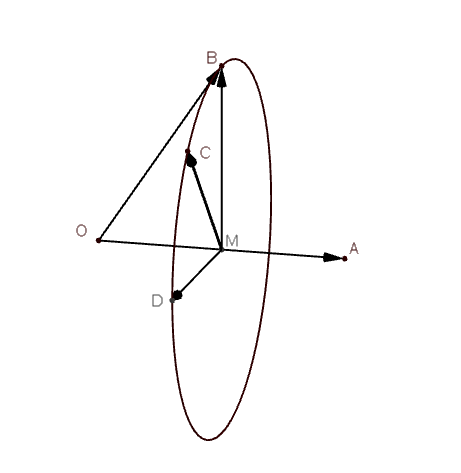
\includegraphics[width=0.3\textwidth]{./img/pic1.png} % 图片路径
    \end{figure}

为了方便, 记 $\lvec{OA} = \mla$, $\lvec{OB} = \mlb$, 记 $\alpha := \angle(\mla, \mlb)$.

设 $\lvec{OB}$ 投影到 $\lvec{OA}$ 上的向量是 $\lvec{OM}$. 将 $\lvec{OB}$ 逆时针旋转 $\frac{\pi}{2}$ 得到的向量为 $\lvec{OD}$. 那么在 $BMD$ 这个平面上, $\lvec{MC}$ 可以轻松用 $\lvec{MB}$ 和 $\lvec{MD}$ 表示为
\[
    \lvec{MC} = \cos \theta \lvec{MB} + \sin \theta \lvec{MD},
\]
接下来只需要计算 $\lvec{OM}$, $\lvec{MB}$ 和 $\lvec{MD}$ 即可.
\[
    \lvec{OM} = \frac{\mla \cdot \mlb}{|\mla|^2}\mla,
\]  
\[
    \lvec{MB} = \mlb - \lvec{OM} = \mlb - \frac{\mla \cdot \mlb}{|\mla|^2}\mla.
\]
设 $\lvec{MD} = k \mla \times \mlb$, 根据 $|\lvec{MD}| = |\lvec{MB}|$ 可以列出方程
\[
    k |\mla| |\mlb| \sin \alpha = |\lvec{MD}| = |\lvec{MB}| = |\mlb| \sin \alpha,
\] 
得到
\[
    k = \frac{1}{|\mla|},
\]
所以
\[
    \lvec{MD} = \frac{\mla \times \mlb}{|\mla|}.
\]
那么
\[
    \lvec{MC} = \cos \theta \left(\mlb - \frac{\mla \cdot \mlb}{|\mla|^2}\mla\right) + \sin \theta \frac{\mla \times \mlb}{|\mla|},
\]
因此
\[
    \lvec{OC} = \frac{\mla \cdot \mlb}{|\mla|^2}\mla + \cos \theta \left(\mlb - \frac{\mla \cdot \mlb}{|\mla|^2}\mla\right) + \sin \theta \frac{\mla \times \mlb}{|\mla|},
\]
即
\[
    \lvec{OC} = \frac{\mla \cdot \mlb}{|\mla|^2}(1 - \cos \theta)\mla + \cos \theta \mlb + \sin \theta \frac{\mla \times \mlb}{|\mla|}.
\]
\end{solution}

\subsection*{ 123页 题目1(1) (4) }
\begin{problem*}
题目略
\end{problem*}
\begin{solution}
\begin{enumerate}
    \item[(1)] $|(\mla, \mlb, \mlc)| = |(\mla \times \mlb) \cdot \mlc| \leqslant |\mla \times \mlb||\mlc| \leqslant |\mla||\mlb||\mlc|$. 几何意义就是说, 在三组边长固定了的所有平行六面体中, 长方体的体积最大.
    \item[(4)] 我们先证明 (2), 即混合积关于第三个元素是线性的.
    \begin{proof}
        \[
        \begin{aligned}
            (\mla, \mlb, \lambda \mlc + \mu \mld) ={}& (\mla \times \mlb) \cdot (\lambda \mlc + \mu \mld) \\
            ={}& (\mla \times \mlb) \cdot \lambda \mlc + (\mla \times \mlb) \cdot \mu \mld \\
            ={}& \lambda (\mla, \mlb, \mlc) + \mu (\mla, \mlb, \mld).
        \end{aligned}
        \]
        同时, 由于混合积交换后只变符号, 所以混合积对第一、第二位元素也是线性的.
    \end{proof}
    回到原题. 利用线性性将 $(\mla, \mlb, \mlc)$ 展开, 一共有 $9$ 项, 可以表示为
    \[
        (\mla, \mlb, \mlc) = \sum_{i, j, k = 1}^{3} a_ib_jc_k (e_i, e_j, e_k),
    \]
    而如果 $i, j, k$ 中有两个一样, 那么 $(e_i, e_j, e_k) = 0$. 所以只有三个各不相同的时候, 才可能出现非零的求和式. 因此上述求和可以改为
    \[
        (\mla, \mlb, \mlc) = \sum_{ijk \text{是} 3-\text{排列}} a_ib_jc_k (e_i, e_j, e_k),
    \]
    因为 $ (e_i, e_j, e_k) = (-1)^{\tau(ijk)}(e_1, e_2, e_3)$, 所以
    \[
        (\mla, \mlb, \mlc) = \sum_{ijk \text{是} 3-\text{排列}} (-1)^{\tau(ijk)}a_ib_jc_k (e_1, e_2, e_3),
    \]
    而 $\sum_{ijk 是 3-排列} (-1)^{\tau(ijk)}a_ib_jc_k$ 就是题目中的行列式, 因此
    \[
        (\mla, \mlb, \mlc) = \left|\begin{matrix}
            a_1 & a_3 & a_3 \\
            b_1 & b_3 & b_3 \\
            c_1 & c_3 & c_3 \\
        \end{matrix}\right| (e_1, e_2, e_3).
    \]
\end{enumerate}
\end{solution}

\subsection*{ 题目2 (1) }
\begin{problem*}
已知四点坐标, 判断是否共面. 如果不共面, 求出四面体体积和从顶点 $D$ 引出的高.
\[
A(1, 0, 1), B(4, 4, 6), C(2, 2, 3), D(10, 14, 17).
\]
\end{problem*}
\begin{solution}
作差
\[
\lvec{AB} = (3, 4, 5), \quad \lvec{AC} = (1, 2, 2), \quad \lvec{AD} = (9, 14, 16),
\]
计算混合积(行列式)为
\[
\left|
\begin{matrix}
    3 & 4  & 5 \\
    1 & 2  & 2 \\
    9 & 14 & 16
\end{matrix}
\right| = 0,
\]
为零, 所以共面. 
\end{solution}

\subsection*{ 题目4 (2) }
\begin{solution}
\[
(\mla \times \mlb) \times \mlc = (\mla \cdot \mlc) \mlb - (\mlb \cdot \mlc) \mla = 7\mlb - 20\mla = (-46, 29, -12).
\]
\end{solution}

\subsection*{ 题目 5(1)(5) }
\begin{solution}
\begin{enumerate}
    \item[(1)]
    \[
    \begin{aligned}
        \mlb \cdot [(\mla \times \mlb) \times \mla]  ={}& \mlb \cdot [(\mla \cdot \mla)\mlb - (\mlb \cdot \mla)\mla] \\
        ={}& (\mla \cdot \mla)(\mlb \cdot \mlb) - (\mla \cdot \mlb)^2 \\
        ={}& |\mla|^2|\mlb|^2(1 - \cos^2 \angle(\mla, \mlb)) \\
        ={}& |\mla|^2|\mlb|^2\sin^2 \angle(\mla, \mlb).
    \end{aligned}
    \]
    \item[(5)] ``$\Rightarrow$'': 如果三个向量共面, 那么他们的叉乘都和三个向量所在的那个平面垂直, 所以三个叉乘向量共线.(如果三个向量还是共线的, 那么叉乘为 0, 所以结论也成立);
    ``$\Leftarrow$'': 如果三个叉乘共面, 那么
    \[
    \begin{aligned}
        0 = (\mlb \times \mlc, \mlc \times \mla, \mla \times \mlb) ={}& 
        [(\mlb \times \mlc) \times (\mlc \times \mla)] \cdot (\mla \times \mlb) \\
        ={}& \{[\mlb \cdot (\mlc \times \mla)]\mlc - [\mlc \cdot (\mlc \times \mla)]\mlb\} \cdot (\mla \times \mlb) \\
        ={}& [\mlb \cdot (\mlc \times \mla)]\mlc \cdot (\mla \times \mlb) \\
        ={}& (\mlc, \mla, \mlb)(\mla, \mlb, \mlc) \\
        ={}& (\mla, \mlb, \mlc)^2 = 0,
    \end{aligned}
    \]
    因此原来的三个向量共面.
\end{enumerate}
\end{solution}